\documentclass[11pt]{article}
\usepackage[preprint]{acl}
\usepackage{times}
\usepackage{latexsym}
\usepackage[T1]{fontenc}
\usepackage[utf8]{inputenc}
\usepackage{microtype}
\usepackage{booktabs}
\usepackage{amsmath}
\usepackage{graphicx}
\usepackage{multirow}
\usepackage{xcolor}

\title{Memory Rewrites Do Not Drift, They Collapse:\\ Detecting and Guarding Against Catastrophic Consolidation\\ in Long-Term LLM Agent Memory}

\author{Selvin PaulRaj K \\
  Department of Computer Science and Engineering \\
  Kings Engineering College, Chennai, India}

\begin{document}
\maketitle

\begin{abstract}
LLM-rewritten agent memory does not erode a little with every rewrite. It fails abruptly. Across LoCoMo, Memora and LongMemEval, repeatedly rewriting fixed content loses facts once and then holds a fixed point, but a 30B writer occasionally \emph{collapses}: one rewrite discards at least half of the memory. Collapses hit 6 of 19 LoCoMo and Memora streams and 21 of 23 LongMemEval streams, where about one rewrite in six collapsed. A 550B writer from the same family did not collapse in our 293 rewrites. Collapses are visible as a sharp length drop, and on collapsed rewrites only 11.6\% of memory lines survive, against 96.2\% otherwise. A retry triggered by this signal raised accuracy on five of the six collapsed units, but at the level of conversations and personas no guard effect survives multiple-comparison correction, and on LongMemEval the guard hurt. We argue that memory systems should monitor per-rewrite length, not average accuracy.
\end{abstract}

\section{Introduction}
Long-term conversational agents cannot keep every past session in context, so many systems keep a consolidated memory that an LLM edits as new sessions arrive \citep{packer2023memgpt,chhikara2025mem0,xu2025amem,rasmussen2025zep}. Each rewrite is lossy, so a natural hypothesis is that errors compound: facts erode a little with every pass until the memory no longer reflects the user. Recent work reports that consolidated memories can become faulty under continuous updates \citep{zhang2026faulty} and that compaction loses exact-wording rules over rounds \citep{zerhoudi2026cliff}.

We set out to measure this drift curve directly and did not find it. We found a different failure mode with a different remedy. Most rewrites preserve or grow the memory; a few discard most of it in one step. These \emph{collapses} are invisible in averages over many users, yet they cause the worst per-user outcomes, such as a memory that ends with ``dogs' names: not explicitly listed'' after earlier notes had named all three dogs.

\textbf{Contributions.}
\begin{itemize}
\item A controlled measurement of rewrite drift on LoCoMo \citep{maharana2024locomo} and Memora \citep{uddin2026memora}. Fixed-content rewriting loses facts once and then reaches a fixed point. Streaming rewrites are not significantly different from append-only notes on average (\S\ref{sec:drift}).
\item The characterisation of \emph{rewrite collapse}: rare single-step losses of at least half of the memory. We report rates, threshold sensitivity, recovery, a second writer model, and a third benchmark, LongMemEval \citep{wu2024longmemeval} (\S\ref{sec:collapse}).
\item A length-triggered \emph{collapse guard}, a bounded variant that removes the memory-size confound, and exploratory controls (keep the old memory, always preserve, no cap, escalate to a larger writer). We report its limits: its gains are concentrated on six collapsed units and are not significant at the unit level, and on LongMemEval it did not help (\S\ref{sec:guard}, \S\ref{sec:explore}).
\item Two practical analyses: whether adding retrieved raw turns to the guarded memory helps (\S\ref{sec:hybrid}), and the context and compute cost of each memory design (\S\ref{sec:cost}).
\end{itemize}
Code, prompts, per-question scores and analysis scripts are released.\footnote{\url{https://github.com/selvin-paul-raj/M.E-Thesis} (folder \texttt{drift-memory}).}

\section{Related Work}
\textbf{Agent memory.} MemGPT \citep{packer2023memgpt}, Mem0 \citep{chhikara2025mem0}, A-Mem \citep{xu2025amem} and Zep \citep{rasmussen2025zep} maintain external memories that an LLM updates. REALM revisits stored memories when they are recalled and reports gains on LoCoMo and LongMemEval \citep{song2026realm}. LoCoMo \citep{maharana2024locomo}, LongMemEval \citep{wu2024longmemeval} and Memora \citep{uddin2026memora} evaluate recall, temporal reasoning and knowledge updates over many sessions; Memora also scores whether agents rely on outdated memories.

\textbf{Degradation under rewriting.} \citet{zhang2026faulty} show that memory utility first rises and then degrades as LLM consolidation proceeds, and they recommend gating consolidation. \citet{zerhoudi2026cliff} show that compaction keeps 53\% of safety rules after one round and 10\% after five, and they propose type-aware compaction. \citet{colaco2026rd} frame compaction as a rate--distortion trade-off and note that the repeated compaction agents perform is almost never measured. \citet{dongre2025drift} model multi-turn context drift as a bounded stochastic process and observe stable, noise-limited equilibria rather than runaway degradation. We see the same equilibrium for fixed content. Our distinct observation is that, in streaming conversational memory, the harmful losses are discrete events that a length signal detects, so a gate needs no classifier and no second model.

\section{Problem Setup}\label{sec:setup0}
A conversation arrives as sessions $s_1,\dots,s_T$. A \emph{streaming} memory starts empty, $M_0=\emptyset$, and after each batch of sessions an LLM writer produces $M_t = W(M_{t-1}, s_t)$, a full rewrite that adds, updates, removes and merges facts under a nominal word budget. A reader answers questions from $M_T$ alone. Let $|M|$ be the word count. We call step $t$ a \textbf{collapse} when
\begin{equation}
|M_{t-1}| \ge L_{\min} \quad\text{and}\quad |M_t| \le \rho\,|M_{t-1}|,
\end{equation}
with $\rho{=}0.5$ and $L_{\min}{=}300$ words, fixed before any guard experiment. A collapse \emph{recovers} if some later $|M_{t'}| \ge |M_{t-1}|$. Note that length recovery does not mean the discarded facts come back; later sessions add new facts.

\section{Experimental Setup}\label{sec:setup}
\textbf{Data.} \emph{LoCoMo}: all 10 conversations (19--32 sessions each). Per conversation we sample 10 questions, stratified by category, whose evidence is at least 5 sessions old (adversarial category excluded). \emph{Memora}: 9 personas from the weekly split, 10 questions each, scored with Memora's rubric checks (442 checks). Sessions are fed in batches of 10. \emph{LongMemEval-S} (cleaned release): 30 instances, about 48 sessions each, stratified by type (multi-session 8, knowledge-update 8, temporal reasoning 8, single-session-user 6; abstention items excluded; seed 13). Sessions are fed in batches of 5, and assistant turns are truncated to 300 characters.

\textbf{Memory arms.} \emph{k0}: append-only notes extracted from each session, never rewritten. \emph{k}$_n$: the full k0 memory rewritten $n$ times (fixed content). \emph{stream}: after each batch, the writer rewrites the whole memory with a nominal 1,200-word cap. \emph{Guards} (\S\ref{sec:guard}) and \emph{raw}/\emph{hybrid} retrieval arms (\S\ref{sec:hybrid}) are defined where they are used. All prompts are in Appendix~\ref{app:prompts}.

\textbf{Models.} Main writer and reader: Nemotron-3.5-Lightning-30B-A3B with reasoning disabled, temperature 0. Second writer: Nemotron-3-Ultra-550B-A55B, with the reader kept fixed so that differences come from the memory. Judge: gpt-oss-120b, scoring each answer against the gold answer (LoCoMo, LongMemEval) or each rubric check (Memora). Early pilots used gpt-oss-20b and Qwen3.8-27B as writers.

\textbf{Statistics.} Accuracy is the share of correct items. Because questions within a conversation share one memory, the unit of inference is the conversation (LoCoMo) or persona (Memora). We report the difference of pooled accuracies with a 95\% unit-level bootstrap interval (10,000 resamples, seed 0; \citealp{efron1994bootstrap}) and an exact sign-flip permutation $p$ over per-unit differences. The two confirmatory guard contrasts (bounded guard vs.\ stream on held-out LoCoMo and pooled) are Holm-corrected. Equivalence uses a two one-sided test with a 5-point margin. A LongMemEval instance has one question, so there question and unit coincide. Collapse rates per stream carry Clopper--Pearson intervals. Contrasts not in the confirmatory family are exploratory.

\section{No Compounding Drift}\label{sec:drift}
\textbf{Fixed content.} In the LoCoMo pilot (30 questions, gpt-oss-20b writer), one rewrite cut memory from 1,129 to 684 words and kept 79\% of k0 facts. Rounds 2--8 changed length and fact survival by at most 1--2\%, and accuracy stayed within 30.0--36.7\% for $k{=}0$ to 8. A small Memora pilot (2 personas, 20 questions, Qwen writer) fell from 58.3\% at $k{=}0$ to 49.5\% at $k{=}2$ and was identical at $k{=}4$ and $k{=}8$. The loss is front-loaded and then stops. The kill-switch we had set for a compounding curve was not met in either pilot: both curves were flat after the first round.

\textbf{Streaming.} With Nemotron on all 9 Memora personas, k0, k$_2$ and stream scored 47.5, 48.2 and 50.9 (stream$-$k0 +3.4 [$-$7.4, +14.6], $p{=}0.68$). Two rewrites of fixed content are equivalent to k0 within 5 points (k$_2-$k0 +0.7 [$-$4.4, +5.8]). On held-out LoCoMo, stream averaged 18.0 against 26.0 for k0 ($p{=}0.16$), and the whole gap came from three conversations (\S\ref{sec:collapse}). Pooled over 19 units, stream$-$k0 was +1.3 [$-$8.1, +10.3]. Averages therefore show no steady erosion.

\section{Rewrite Collapse}\label{sec:collapse}
\textbf{Rate.} Over 19 Nemotron streams (9 Memora, 10 LoCoMo) and 351 rewrites, 13 rewrites collapsed (3.7\%): 4 of 89 on Memora and 9 of 262 on LoCoMo. These hit 6 of 19 streams (95\% CI 13--57\%; 3 of 9 on Memora, 3 of 10 on LoCoMo). Typical events shrank memories from 1,479 to 149 words or from 929 to 220.

\textbf{Collapses are a separate mode, not a tail.} Of the 280 rewrites that started from at least 300 words, 256 kept more than 90\% of the length, 7 kept 70--90\%, 4 kept 50--70\%, and 13 kept at most 50\% (Figure~\ref{fig:thresh}b). The distribution is bimodal: a large mass near 1.0 and a separate cluster at 0.1--0.4. Event counts move smoothly with the threshold (7 events at $\rho{=}0.3$, 19 at $\rho{=}0.7$ with a 200-word floor), and the set of affected streams barely changes (5--6 of 19; Figure~\ref{fig:thresh}a, Table~\ref{tab:thresh}). Our conclusions do not depend on the exact threshold.

\textbf{Not a cap artefact.} The writer is asked to stay under 1,200 words, so a collapse might be the writer obeying the cap. Over all 552 30B rewrites from $\ge$300 words (including LongMemEval), the collapse rate was 10.9\% for memories of 300--600 words, 15.3\% at 600--900, 12.2\% at 900--1,200, 20.8\% at 1,200--1,500 and 6.3\% above 1,500. The median memory length before a collapse was 891 words, and 23 of 52 collapses started at or above 1,000 words. Collapses occur well below the cap; the cap is not their sole cause. A no-cap control appears in \S\ref{sec:explore}.

\textbf{Collapses lose facts, not just words.} We replayed the 280 cached rewrites of the 19 plain 30B streams that started from $\ge$300 words and counted a memory line as surviving if some new line shares at least 60\% of its content tokens (a lexical proxy, not a semantic judgement). On the 13 collapsed rewrites, mean line survival was 11.6\%; on the other 267 it was 96.2\%. A survival threshold of 0.5 flags all 13 collapses (13 of 13 flagged are collapses) and 6 further fact-losing rewrites that shrank only to 0.55--0.86 of their length, which the length rule misses.

\begin{figure}[t]
\centering
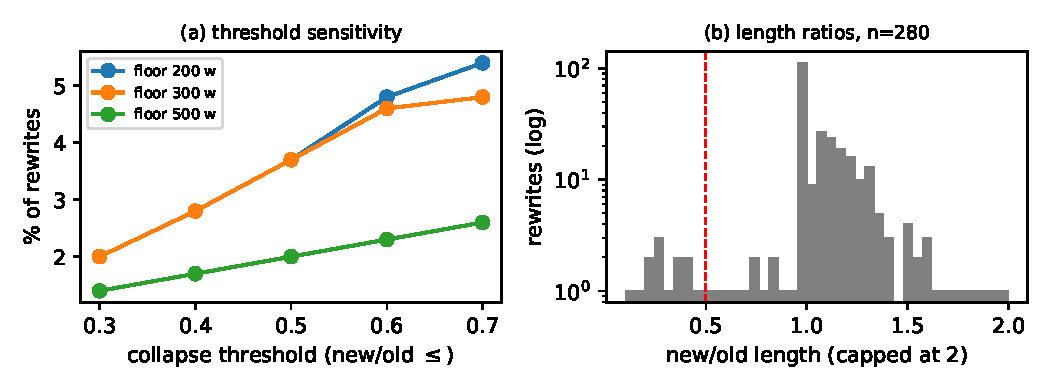
\includegraphics[width=\columnwidth]{fig_threshold.pdf}
\caption{(a) Share of rewrites flagged as collapses for different thresholds $\rho$ and length floors. (b) Distribution of new/old length over 280 rewrites that started from $\ge$300 words (log scale). The red line marks $\rho{=}0.5$.}
\label{fig:thresh}
\end{figure}

\begin{table}[t]
\centering\small
\begin{tabular}{lrrr}
\toprule
$\rho$ & floor 200 & floor 300 & floor 500 \\
\midrule
0.3 & 7 (2.0) & 7 (2.0) & 5 (1.4) \\
0.4 & 10 (2.8) & 10 (2.8) & 6 (1.7) \\
0.5 & 13 (3.7) & \textbf{13 (3.7)} & 7 (2.0) \\
0.6 & 17 (4.8) & 16 (4.6) & 8 (2.3) \\
0.7 & 19 (5.4) & 17 (4.8) & 9 (2.6) \\
\bottomrule
\end{tabular}
\caption{Collapse events (\% of 351 rewrites) by threshold. Bold: the default used throughout.}
\label{tab:thresh}
\end{table}

\textbf{Recovery.} Only 5 of the 13 collapses were later followed by a memory at least as long as before. These were all on LoCoMo (conv-26 after 2 sessions, conv-42 after 12, and conv-47 three times after 4, 10 and 5 sessions). All 4 Memora collapses never recovered, and three streams ended at 89--342 words. Recovery is in length only. In conv-47 the stream collapsed four times; its final memory says the user's dogs' names are ``not explicitly listed, but previously mentioned'', while the k0 notes for the same conversation name Ned, Max and Daisy. Figure~\ref{fig:traj} shows the length trajectories.

\begin{figure}[t]
\centering
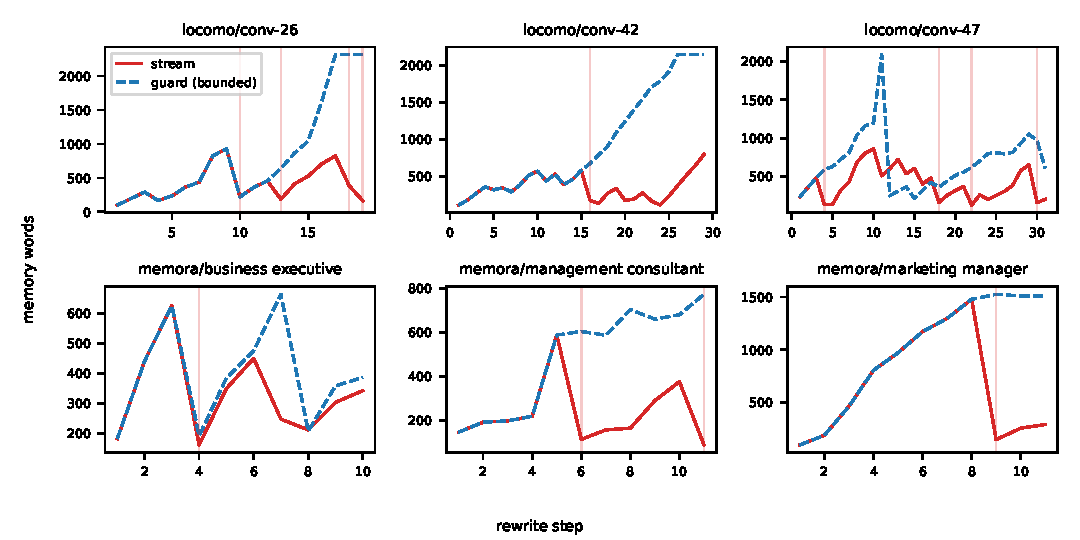
\includegraphics[width=\columnwidth]{fig_trajectories.pdf}
\caption{Memory length per rewrite for all 19 Nemotron streams; collapse events are marked.}
\label{fig:traj}
\end{figure}

\textbf{Damage.} On the three collapsed held-out LoCoMo conversations, stream accuracy was 3.3\% against 23.3\% for k0 ($-$20.0 [$-$36.7, $-$6.7], $p{=}0.001$). On the other seven, the arms were close. On Memora, the three collapsed personas averaged 41.9 for stream against 49.0 for k0, a gap hidden inside a non-significant mean.

\textbf{Other writers and environments.} The pilot writer gpt-oss-20b collapsed as well (4 events on one LoCoMo conversation). With the larger Nemotron-3-Ultra-550B-A55B writer and the same reader, \emph{no} rewrite collapsed in 293 rewrites over 12 streams (all 10 LoCoMo conversations and 2 Memora personas; final memories 1,530--2,298 words). The guard therefore never fired, and guarded and plain streams scored the same (LoCoMo 39.0, Memora 85.0). On LoCoMo the larger writer's plain stream beat the 30B writer's by 21.0 points ([+11.0, +30.0], $p{<}0.001$) with the reader held fixed. At the conversation level this gap is +21.0 [+6.0, +34.0], $p{=}0.031$, with 8 of 10 conversations better. Collapse therefore depends on the writer and is not inherent to rewriting; the 550B writer did not collapse in our runs (0 of 12 streams, 95\% CI 0--26\%). With two writers from one family, we do not claim a scaling trend. On LongMemEval-S, with roughly 48 sessions per instance and the 30B writer, collapse was far more common: 39 of 224 rewrites (17.4\%, about one in six) in 21 of 23 completed instances (95\% CI 72--99\%), with only 11 of 39 regaining their earlier length. Longer, more topically scattered histories make collapse a frequent event rather than a rare one.

\section{A Collapse Guard}\label{sec:guard}
A collapse has a simple signature, a large drop in length, so we guard against it when it happens. When a rewrite collapses, we re-issue it once with an explicit instruction to keep every existing fact unless the new session contradicts or retires it (Appendix~\ref{app:prompts}).
\begin{itemize}
\item \textbf{Guard-append}: if the retry also collapses, keep the old memory and append the new rewrite under ``Recent updates''.
\item \textbf{Guard-bounded}: keep the longer of the two attempts and never append.
\end{itemize}
When no collapse occurs, both guards are identical to stream. Guard-append was designed after seeing the Memora collapses. We then fixed the rule and ran it on all 10 LoCoMo conversations as a held-out test. Guard-append can let memory grow without bound: on two LoCoMo conversations it reached 11,707 and 18,322 words, which confounds accuracy with memory size. Guard-bounded removes that confound. Its largest memory was 2,318 words, within the range of uncollapsed plain streams (up to 2,372).

\begin{table}[t]
\centering\small
\setlength{\tabcolsep}{4pt}
\begin{tabular}{lrrrr}
\toprule
 & k0 & stream & g-app. & g-bnd. \\
\midrule
Memora & 47.5 & 50.9 & 56.8 & 55.2 \\
\quad collapsed (3) & 49.0 & 41.9 & 58.7 & 54.2 \\
LoCoMo, held-out & 26.0 & 18.0 & 26.0 & 24.0 \\
\quad collapsed (3) & 23.3 & 3.3 & 30.0 & 23.3 \\
Pooled (190 q) & 43.5 & 44.8 & 51.1 & 49.4 \\
\bottomrule
\end{tabular}
\caption{Accuracy (\%). g-app.\ and g-bnd.\ are the appending and bounded guards. Collapsed rows are the units whose plain stream collapsed.}
\label{tab:main}
\end{table}

\begin{table}[t]
\centering\small
\setlength{\tabcolsep}{3pt}
\begin{tabular}{llrr}
\toprule
Contrast & Units & $\Delta$ [95\% CI] & $p$ \\
\midrule
g-bnd.$-$stream & LoCoMo (10) & +6.0 [0.0, +13.0] & .25$^\dagger$ \\
g-bnd.$-$stream & Pooled (19) & +4.6 [0.0, +11.0] & .06$^\dagger$ \\
g-bnd.$-$stream & Memora (9) & +4.3 [$-$0.9, +12.1] & .50 \\
g-bnd.$-$stream & Collapsed (6) & +13.5 [+1.2, +28.6] & .06 \\
g-app.$-$stream & Pooled (19) & +6.3 [+1.6, +12.7] & .03 \\
g-app.$-$stream & Collapsed (6) & +18.4 [+10.0, +30.0] & .03 \\
g-bnd.$-$k0 & Pooled (19) & +5.9 [$-$5.4, +16.3] & .63 \\
\bottomrule
\end{tabular}
\caption{Unit-level contrasts (points): conversation or persona bootstrap interval and exact sign-flip permutation $p$. $^\dagger$Confirmatory family; Holm-adjusted $p$ = .25 and .13, neither significant. Other rows are exploratory; the appending guard is confounded with memory size.}
\label{tab:contrast}
\end{table}

\textbf{Results.} Tables~\ref{tab:main} and~\ref{tab:contrast} report accuracy and contrasts. On the held-out LoCoMo replication the bounded guard was 6.0 points above plain streaming, all of it from the three collapsed conversations (+20.0); the other seven are identical by construction. Treating questions as independent, this gap would look significant ($p{=}0.002$), but with conversations as the unit it is not ($p{=}0.25$, Holm-adjusted), because only three units differ. Pooled over both benchmarks the bounded guard won on 5 of the 6 units where it changed anything ($p{=}0.06$; Holm-adjusted 0.13). We therefore read the guard as a consistent repair on the few collapsed units, not as an established average improvement. A single retry recovered 12 of 16 bounded-guard triggers (75\%), where recovery means keeping at least half of the old length. The guard counts more triggers (16) than plain streaming has collapses (13) because, once a retry changes the memory, the guarded stream follows its own trajectory and meets different rewrites; the same holds on LongMemEval (48 triggers vs.\ 39 collapses). The bounded guard gives up 1.7 points against the appending guard. That gap is the price of keeping memory bounded, and the bounded guard is the variant we recommend. Pooled over both benchmarks, the bounded guard is the best bounded-size arm, but it does not significantly beat append-only notes (+5.9, $p{=}0.63$).

\textbf{Per-unit view.} Table~\ref{tab:units} lists the six collapsed units. The bounded guard helps on five and hurts on one (Memora business\_executive, 35.6 $\rightarrow$ 31.1), where the retry also collapsed and the longer attempt was still short. The appending guard handles that case better, which is the expected trade-off.

\begin{table}[t]
\centering\small
\setlength{\tabcolsep}{3.5pt}
\begin{tabular}{lrrrr}
\toprule
Unit & k0 & stream & g-app. & g-bnd. \\
\midrule
LoCoMo conv-26 & 20.0 & 0.0 & 30.0 & 10.0 \\
LoCoMo conv-42 & 30.0 & 10.0 & 40.0 & 40.0 \\
LoCoMo conv-47 & 20.0 & 0.0 & 20.0 & 20.0 \\
Memora bus.\ exec. & 55.6 & 35.6 & 46.7 & 31.1 \\
Memora mgmt.\ cons. & 58.2 & 49.1 & 56.4 & 56.4 \\
Memora mkt.\ mgr. & 34.5 & 40.0 & 70.9 & 70.9 \\
\bottomrule
\end{tabular}
\caption{Accuracy (\%) on the six units whose plain stream collapsed.}
\label{tab:units}
\end{table}

\textbf{LongMemEval: the guard does not transfer.} We ran the bounded guard unchanged on LongMemEval-S (23 of 30 planned instances completed; 7 runs were lost to provider errors). Here it fired on 48 of 224 rewrites (21.4\%), and the retry kept at least half of the old length in 28 cases. Accuracy did \emph{not} improve: stream 4 of 23 correct (17.4\%), guard 1 of 23 (4.3\%; $-$13.0 [$-$26.1, 0.0], $p{=}0.077$). The guarded memories were longer (mean 1,051 vs.\ 720 words) but answered fewer questions. With 23 questions the interval is wide and touches zero, so we report this as a likely failure case: when collapses are frequent, forcing the writer to keep old content appears to crowd out the knowledge updates and temporal details LongMemEval asks about. The guard is a remedy for rare collapses, not for a writer that collapses on every fifth rewrite.

\section{Exploratory Controls}\label{sec:explore}
The analyses in this section were designed after the main results and before our analysis plan was fixed, so they are exploratory and uncorrected.

\textbf{Escalate instead of retry.} When the 30B rewrite collapses, we re-issue the same prompt once to the 550B writer and keep its output. On the six collapsed units this \emph{escalation guard} scored 56.2 against 35.7 for stream (+20.5 [+3.3, +33.3], $p{=}0.06$; better on 5, tied on 1), but it was not better than the bounded retry (+7.0 [$-$8.0, +27.7], $p{=}1.0$). On 22 LongMemEval instances it answered 3 correctly; like the bounded guard, it did not fix the high-collapse setting.

\textbf{Keep the old memory.} A \emph{floor-reject} variant discards any collapsed rewrite and keeps the previous memory. On the three collapsed LoCoMo conversations it scored 0.0, 10.0 and 10.0 (stream 0.0, 10.0, 0.0; bounded guard 10.0, 40.0, 20.0). Rejecting a rewrite also drops the session it should have added, so it is not a substitute for a retry.

\textbf{Always preserve.} Adding the keep-facts instruction to \emph{every} rewrite did not prevent collapse: LoCoMo conv-26 still fell from 2,276 to 173 words and scored 10.0. On Memora business\_executive it scored 60.0 (stream 35.6, bounded guard 31.1).

\textbf{No cap.} Removing the 1,200-word budget from the prompt did not prevent collapse either: Memora marketing\_manager still fell from 524 to 157 words (38.2; stream 40.0). Together with the length bins in \S\ref{sec:collapse}, this suggests collapse is not just cap compliance. These controls cover only some units; we report them as indications, not results.

\section{Does Raw Evidence Help the Guarded Memory?}\label{sec:hybrid}
A natural extension is to pair the bounded-guard memory with retrieved original turns, so that facts lost in a rewrite can still be found. We test a \emph{hybrid} reader context: the guarded memory plus the BM25 top-$k$ raw turns for the question ($k{=}10$ on LoCoMo and LongMemEval, $k{=}15$ on Memora), against \emph{raw}, the BM25 turns alone. These runs use single-question reads, whereas the earlier sections batch 10 questions per call, so we compare raw and hybrid only with each other.

\begin{table}[t]
\centering\small
\setlength{\tabcolsep}{1.5pt}
\begin{tabular}{lrrr}
\toprule
Subset & raw & hybrid & $\Delta$ [95\% CI], $p$ \\
\midrule
LoCoMo (100 q) & 31.0 & 39.0 & +8.0 [$-$1.0, +17.0], .108 \\
Memora (90 q) & 54.3 & 50.9 & $-$3.4 [$-$10.2, +3.5], .355 \\
Collapsed units & 53.5 & 51.4 & $-$2.2 [$-$12.4, +7.5], .730 \\
LongMemEval (23 q) & 39.1 & 47.8 & +8.7 [$-$8.7, +26.1], .444 \\
\bottomrule
\end{tabular}
\caption{Raw retrieval alone vs.\ guarded memory plus raw retrieval (single-question reads).}
\label{tab:hybrid}
\end{table}

Table~\ref{tab:hybrid} shows no significant gain from the combination. On LoCoMo the hybrid was 8 points ahead but the interval includes zero; on Memora it was 3.4 points behind. Per persona, the hybrid gained on four Memora personas and lost on three (largest loss: sales\_manager, 44.9 $\rightarrow$ 22.4). A longer context with a consolidated summary on top does not reliably help this reader, so we do not claim the hybrid as an improvement. The negative result also bounds the guard's role: it repairs the memory, but it is not a substitute for retrieval when exact wording matters.

\section{Deployment Cost}\label{sec:cost}
Table~\ref{tab:cost} gives the reader context each design produces. The collapse check is a word count and costs no model call. The bounded guard adds one writer call on each trigger: 16 of 351 rewrites (4.6\%) on LoCoMo and Memora. The appending guard triggered on 40 rewrites (11.4\%; 30 fell back to appending), and its memory grew to 18,322 words, so its reader cost is unbounded. The bounded guard's mean reader context (1,291 words) is close to plain streaming (1,070 on Memora, 1,533 on LoCoMo). On LongMemEval, where the guard fired on 21.4\% of rewrites, the writer cost of the bounded guard rises accordingly, and the hybrid context is about three times the size of raw retrieval alone. In tokens (cached usage of 370 30B writer calls), a rewrite averaged 2,302 prompt tokens (max 4,426) and 1,645 completion tokens (max 3,000), so a guard retry costs about 3,900 extra tokens per trigger, or about 180 tokens per rewrite at the 4.6\% trigger rate. We did not compute token counts for the 550B writer.

\begin{table}[t]
\centering\small
\setlength{\tabcolsep}{2.5pt}
\begin{tabular}{llrr}
\toprule
Env. & Arm & mean words & max words \\
\midrule
LoCoMo & k0 & 1,217 & 2,098 \\
LoCoMo & stream & 1,533 & 2,372 \\
LoCoMo & guard-append & 4,634 & 18,322 \\
Memora & k0 & 1,011 & 1,584 \\
Memora & stream & 1,070 & 1,556 \\
Memora & guard-append & 1,494 & 2,252 \\
Both & guard-bounded & 1,291 & 2,318 \\
LongMemEval & stream & 720 & 2,043 \\
LongMemEval & guard-bounded & 1,051 & 2,426 \\
LongMemEval & raw (BM25) & 500 & 689 \\
LongMemEval & hybrid & 1,561 & 2,847 \\
\bottomrule
\end{tabular}
\caption{Reader context size per arm (words). The guard check itself needs no model call.}
\label{tab:cost}
\end{table}

\section{Discussion}
The drift-as-erosion picture predicts a smooth decline that grows with the number of rewrites. Our data show something else: a stable equilibrium punctuated by rare catastrophic events. This has five practical consequences. First, average accuracy is a poor monitor. On Memora, three collapsed personas were hidden inside a non-significant mean. Systems should log memory length per rewrite and report the worst units, not only the mean. Second, collapses are cheap to detect. A word-count ratio needs no extra model call until it fires; the bounded guard re-runs 4.6\% of rewrites and the appending guard 11.4\%. Third, the remedy is local. A retry at the moment of collapse suffices, so the consolidation design does not need replacing. This complements \citet{zhang2026faulty}, who argue for gating consolidation, by giving a concrete, inexpensive trigger. Fourth, the evidence for the guard is thin. Its gains sit on six units and are not significant at the unit level, so it should be evaluated on many more collapsed streams before it is recommended as a default. Fifth, the guard has limits. When the retry also collapses, a bounded guard cannot restore facts. On LongMemEval, where one rewrite in six collapsed, guarding made accuracy worse. The collapse rate itself is the useful monitor: near zero calls for nothing, a few percent calls for a guard, and a high rate calls for a stronger writer (a 550B writer removed collapse entirely in our runs).

\section{Conclusion}
LLM-rewritten agent memory does not erode steadily. It holds a fixed point and occasionally collapses. How often it collapses depends on the writer and the history: never in 293 rewrites with a 550B writer, 3.7\% with a 30B writer on LoCoMo and Memora, and 17.4\% on LongMemEval. When collapses are rare, a length-triggered retry with a bounded fallback repaired five of the six collapsed units, though this is not significant at the unit level. When they are frequent, the guard did not help, and a stronger writer is the better fix. Memory systems should log length per rewrite, guard against rare collapses, and treat a high collapse rate as a sign to change the writer.

\section*{Limitations}
The guard was designed after inspecting the Memora collapses. With conversations or personas as the unit, no guard contrast in the confirmatory family is significant, and the exploratory controls (\S\ref{sec:explore}) were run before our analysis plan was fixed. Only the LoCoMo replication and the LongMemEval run are held out. The bounded variant was introduced after we saw the appending guard's length growth on LoCoMo, although its rule needs no tuning. Samples are small (90 + 100 + 23 questions; 7 planned LongMemEval instances and 7 Memora personas for the second writer were not completed because of provider errors), and collapses occur in few streams, so per-subset intervals are wide. The two main writers come from one model family (Nemotron), run at temperature 0 with one prompt; a second family (Qwen3.8-27B) and a second judge from another family are in progress and not reported here. Other families, prompts and sampling temperatures are untested beyond two pilot writers. The judge is an LLM and has not yet been audited against human labels; strict grading together with frequent ``unknown'' answers lowers absolute LoCoMo accuracy. The 50\%/300-word threshold is a heuristic. Writers exceed the nominal 1,200-word cap, so ``bounded'' means bounded by the writer's own behaviour. All benchmarks use synthetic or simulated dialogues; we did not test with real user logs. On LongMemEval we truncate assistant turns to 300 characters, which removes some answers to assistant-side questions.

\section*{Ethics Statement}
We use only public benchmark data whose dialogues are synthetic or simulated. Memory systems that store personal facts raise privacy concerns. Collapse guards keep facts that would otherwise be dropped, so deletion requests must be honoured explicitly rather than left to lossy rewrites.

\bibliography{refs}

\appendix
\section{Prompts}\label{app:prompts}
\small
\textbf{Streaming update (writer).} \texttt{You maintain a long-term memory for a chat assistant. Update the MEMORY with the NEW SESSION: add new facts (with absolute dates; resolve relative dates using the session date), update or remove facts that changed, merge duplicates, keep it organised and concise, one fact per line starting with '- '. Keep the whole memory under \{cap\} words. Output only the full updated memory. MEMORY: \{mem\} NEW SESSION: \{sess\}}

\textbf{Guard retry prefix.} \texttt{IMPORTANT: the current memory has \{n\} words. Your last attempt shrank it to \{m\} words and lost facts. Keep every existing fact unless the new session explicitly contradicts or retires it; merge new facts in.} (followed by the streaming prompt)

\textbf{k0 extraction.} \texttt{You maintain a long-term memory for a chat assistant. Below are new dialogue sessions (with dates). Write concise memory notes: one fact per line, starting with '- ', covering people, events (with absolute dates), preferences, plans, relationships. Resolve relative dates like 'yesterday' using the session date. Output only the notes.}

\textbf{Fixed-content rewrite (k$_n$).} \texttt{Consolidate the memory below: merge duplicates, resolve conflicts, keep it organised and concise, one fact per line starting with '- '. Keep it under \{cap\} words. Output only the rewritten memory.}

\textbf{Reader.} \texttt{Answer each question using ONLY the context. Be short (a few words or a date). If the context does not contain the answer, write 'unknown'. Reply as JSON.} The hybrid context is formatted as \texttt{CONSOLIDATED MEMORY: \ldots\ RAW EVIDENCE (original messages retrieved for this question): \ldots}

\textbf{Judge.} \texttt{Grade each predicted answer against the gold answer. 1 if it conveys the same information (dates may differ in format), else 0. Reply as JSON.}

\section{Reproducibility}\label{app:repro}
All model calls are cached by prompt hash. Scripts: \texttt{stream\_pilot.py} (streaming), \texttt{a7\_locomo.py} (held-out LoCoMo), \texttt{a8\_retry\_only.py} (bounded guard), \texttt{a9\_analysis.py} (thresholds, recovery, cost), \texttt{a10\_hybrid.py} (raw/hybrid), \texttt{a11\_longmemeval.py} (LongMemEval), \texttt{a13\_second\_writer.py} (second writer), \texttt{boot.py} (question bootstrap), \texttt{a16\_review\_stats.py} and \texttt{stats\_cluster.py} (unit-level inference, collapse rates, length bins), \texttt{a13\_unit\_stats.py}, \texttt{a15b\_escalate.py}/\texttt{a15\_escalate\_lme.py} (escalation), \texttt{a17\_controls.py} (controls), \texttt{a18\_fact\_survival.py} (line survival, token use). Per-question scores are released as CSV files.

\end{document}
